\chapter{Logica dinamica}
 Questa logica cerca di mettere assieme tutti i vantaggi visti del CMOS, dal punto di vista dei consumi, e della logica a rapporto per quanto concerne le dimensioni. 


 La	logica dinamica usa la	memoria dei valori dei segnali insita nei nodi di	uscita (dato che sono dei condensatori) ad	alta impedenza.

\begin{itemize}
    \item Una	volta	caricati,	se	lasciati	liberi	i	nodi	non	si	scaricano	subito;
    \item  Usa	un	solo	transistore	per	ogni	ingresso, rispetto a due della logica CMOS	(più	un	paio	di	servizio)
\end{itemize}


\section{Due fasi}

Il circuito del pull down è identico al CMOS, la quale calcola la funzione. 

Inoltre vi sono due transistori aggiuntivi, $M_p $ e $M_e$ controllati da un degnale CLK (non necessariamente uguale a quello di sistema).

\begin{figure}[htbp]
    \centering
    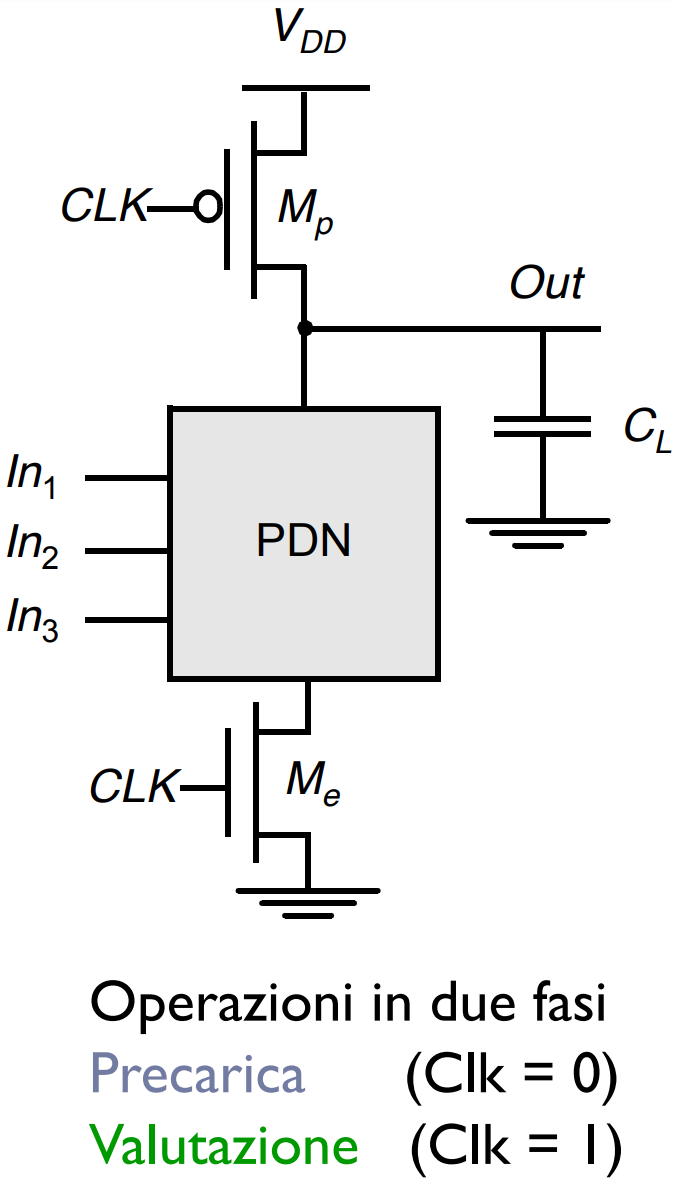
\includegraphics[width=0.25\linewidth]{img/due_fasi.png}
\end{figure}

\subsection{Fase 1: precarica}

Nella fase di precarica il segnale CLK = 0, in questo caso :

\begin{itemize}
    \item il transistore pMOS $M_p$ caricherà la capacità $C_L$ a $V_{DD}$;
    \item il transistore nMOS $M_e$ stacca il PND da massa in modo che non possa influire sulla fase di carica.
\end{itemize}

\newpage
\subsection{Fase 2: valutazione}

Nella fase di valutazione il segnale CLK = 1, in questo caso :

\begin{itemize}
    \item il transistore pMOS $M_p$ si disattiva, mentre $M_e$ si attiva;
    \item se la rete PND conduce (a causa dei valori di ingresso), allora l'uscita viene portata a livello logico basso: 0 V;
    \item se	la	rete	PDN	non	conduce,	l'uscita rimane a	1	grazie	alla carica immagazzinata nel condensatore $C_L$.
\end{itemize}

Dunque ora invece che avere una funzione complessa, numerosi transistori, nel pull-up abbiamo semplificato tutto mettendo un semplice transistore di precarica.


\paragraph{Esempio:}
Precarica: CLK	=	0; L'uscita Out va al	valore 1	qualunque sia il valore degli ingressi A,	B	e	C.

\begin{figure}[htbp]
    \centering
    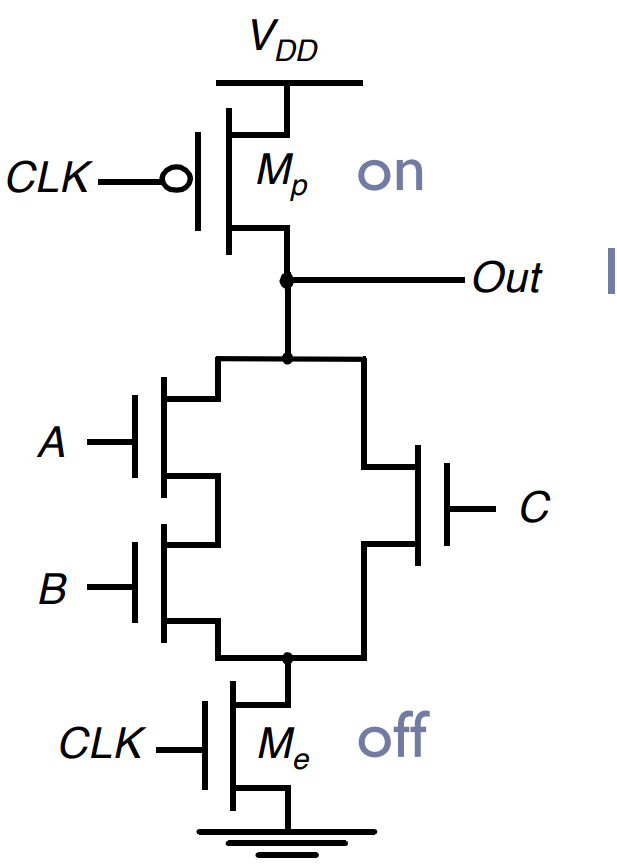
\includegraphics[width=0.26\linewidth]{img/esempio_precarica.png}
    
    
\end{figure}

\paragraph{}
Valutazione: CLK	=	1; Si	abilita $M_e$ e	si disabilita $M_p$; C'è un	collegamento tra Out e	massa se	
e	solo	se	A ·	B	+	C	ha	valore 1, altrimenti l'uscita rimane 1.

\begin{figure}[htbp]
    \centering
    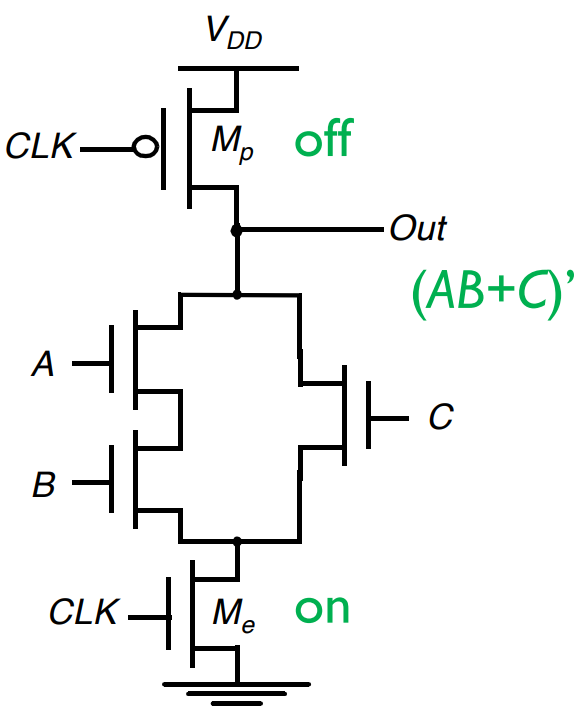
\includegraphics[width=0.27\linewidth]{img/esempio_valutazione.png}
    
    
\end{figure}

In ogni caso la funzione che ci interessa è quella realizzata con CLK = 1: CLK' +	CLK(AB	+	C)'.

\newpage
\section{Condizioni di funzionamento}

Abbiamo visto che ci offre vantaggi dal punto di vista delle dimensioni e da notare anche che non vi è mai un cammino tra $V_{DD}$ e massa, rispetto ad una logica a rapporto, come nel CMOS. Ci sono anche dei lati negativi...

\paragraph{}
Una volta che l'uscita della porta dinamica è	stata scaricata,	non	può essere più caricata fino al	successivo ciclo di	precarica. Quindi i glitch nel pull-down possono avere effetti devastanti.
\paragraph{Conseguenza:} gli ingressi alla porta dinamica possono fare	al	più una transizione durante la	fase di	valutazione.

\paragraph{}

L'uscita si può trovare in	uno stato di	alta impedenza
(nessun transistore che la	pilota, più soggetta a rumore;	di	fatto staccata dal circuito)
\begin{itemize}
    \item[] Sia durante che dopo la	valutazione (PDN	off)
    \item[] Lo	stato è	immagazzinato nella capacità $C_L$
\end{itemize}

\subsection{Proprietà della logica dinamica (pro's)}
\begin{itemize}
    \item[-] La	funzione logica è	realizzata solo	dalla rete	di	pull-down, il	numero di	transistori è	pari a	N	+	2	(contro i	2N	per la	logica statica CMOS);
    \item[-] L'output usa l'intero range	di	valori: $V_{OL} = Gnd$ e	$V_{OH} =	V_{DD}$;
    \item[-] Logica non	a	rapporto, dimensionamento dei dispositivi non	influisce sui	livelli logici;
    \item[-] Commutazione veloce: capacità di	carico ridotta per	il minore numero di	ingressi e	transistori in	uscita;
    \item[-] No	corrente statica, tutta la	corrente fornita da	PDN	è	usata per	scaricare CL.
\end{itemize}

\subsection{Proprietà della logica dinamica (con's)}

\begin{itemize}
    \item[-] Sommando tutto,	il consumo di	potenza è	più elevato che per	la	logica statica CMOS, ma minore della logica a rapporto
     \begin{itemize}
         \item[] No	consumo statico;
         \item[] L'uscita commuta con	più facilità (se	fosse	sempre a	0,	commuta lo	stesso);
         \item[] Il	clock	ha	un	carico ulteriore.
     \end{itemize}
\end{itemize}

\begin{itemize}
    \item[-]  La	rete	di	pull-down	comincia a	lavorare appena il segnale di	ingresso eccede $V_{TN}$
     \begin{itemize}
         \item[] Quindi $V_{IH}$ e	$V_{IL}$ sono uguali a	$V_{TN}$
         \item[] I	margini di	rumore sono più ridotti ($NM_L$)
     \end{itemize}
\end{itemize}

 \begin{itemize}
     \item[-] Richiede un	ciclo di	precarica/valutazione
      \begin{itemize}
          \item[] Controllo	più	complesso
          \item[] Il	periodo	del	ciclo	non	può	superare	un	certo	valore,	altrimenti	lo	stato	viene	perso	a	causa	delle	correnti	di	leakage
      \end{itemize}
 \end{itemize}

\section{Cascata di porte dinamiche}

 Mentre in CMOS è molto semplice usare porte in cascata, nella logica dinamica invece è difficile	realizzare cascate di	porte.
 \paragraph{Esempio:} Durante	la	precarica le	uscite dei due	inverter	vanno entrambe a	$V_{DD}$. 

 
 Supponiamo l'ingresso In vada a	1: all'inizio della fase di	valutazione l'uscita Out1 comincia a	scaricarsi, mentre Out2 dovrebbe rimanere a	1.

 
 Però c'è un	tempo	durante il quale	l'ingresso del	secondo	inverter	è ancora a	1 e anche Out2 comincia a	scaricarsi
fino a	quando Out1 non	scende sotto	$V_{TN}$. 
 Non	si può recuperare il livello
perso,	e	si rischiano
malfunzionamenti.

\begin{figure}[htbp]
    \centering
    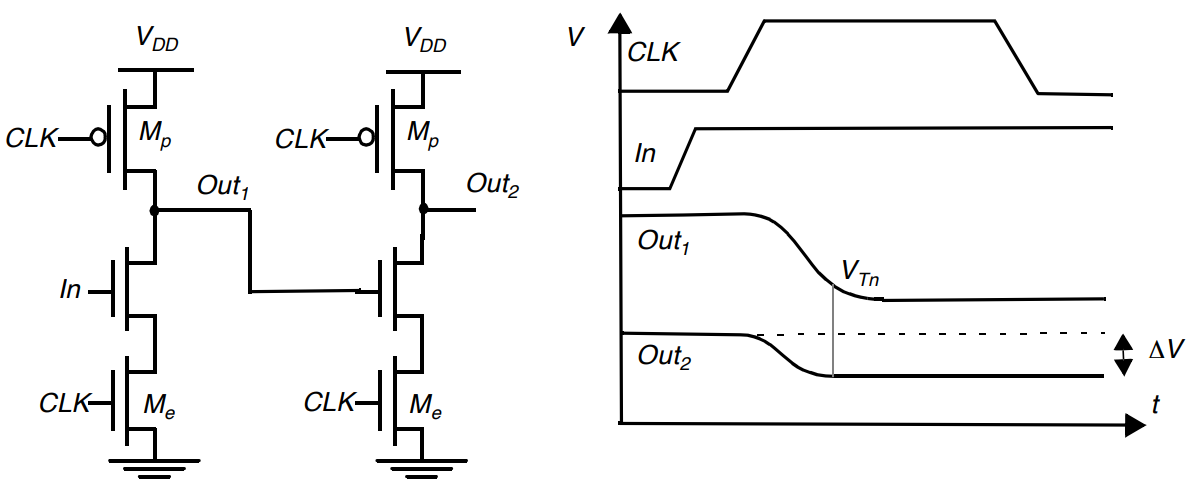
\includegraphics[width=0.6\linewidth]{img/es_cascata.png}    
    
\end{figure}

\newpage
\subsection{Logica domino}
Per	operare correttamente,	gli ingressi dovrebbero solo	fare	transizioni da	0	a	1	durante la	valutazione, in	questo modo non	si rischia di	attivare per	errore la	PDN.

La	logica domino	inserisce un	inverter	dopo ogni porta, e grazie a ciò si potranno fare solo transizioni da 0 a 1: le	uscite quindi sono inizialmente a	0	durante la	precarica, ed	eventualmente vanno a	1	se	si attiva la	PDN.


\begin{figure}[htbp]
    \centering
    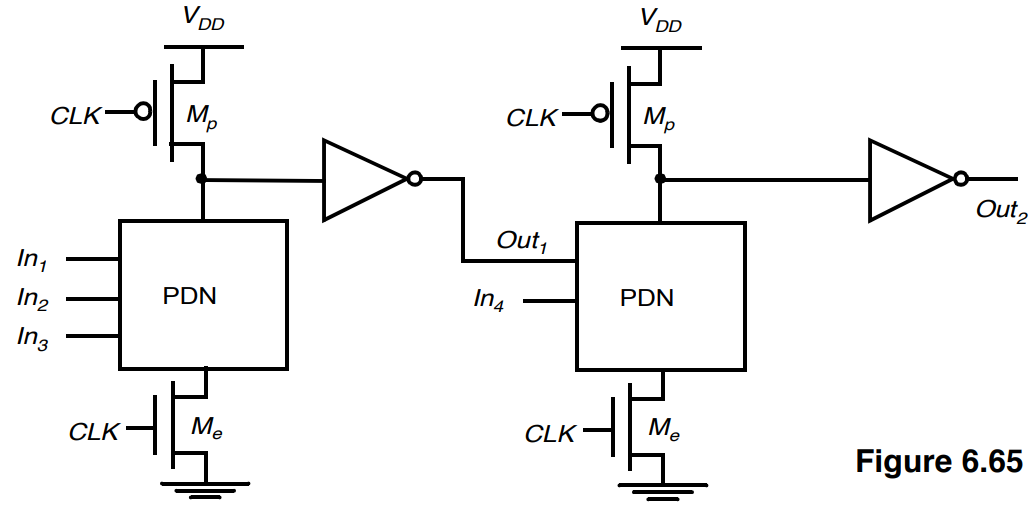
\includegraphics[width=0.6\linewidth]{img/logica_domino.png}
    
    
\end{figure}

Facendo così però, la PDN da invertente, introducendo l'inverter,	la	logica domino	permette di	realizzare solo	funzioni non	invertenti. Questo è un grande svantaggio in quanto non si possono realizzare tutte le porte logiche, AND e OR, che sono le due porte non invertenti, non costituiscono un insieme  completo di operatori, serve anche la NOT.


\section{Altre logiche: take away}

Abbiamo visto varie soluzioni per la costruzione di porte logiche:

\begin{itemize}
    \item[-] Logiche	a	rapporto;
    \item[-] Pass	transistor;
    \item[-] Logiche	dinamiche.
\end{itemize}

con vari compromessi: 
\begin{itemize}
    \item[] range dei livelli;
    \item[] i consumi;
    \item[] margini di rumore;
    \item[] velocità;
    \item[] rumore.
\end{itemize}

Ovviamente nulla viete di usare un mix di modelli per la costruzione: usare CMOS dove servono consumi ridotti a scapito delle dimensioni; logica dinamica quando non abbiamo problemi di interconnessioni e sappiamo che gli ingressi non variano così spesso; parti con pass transistor e transistor gate come ad esempio i multiplexer i quali vengono molto semplici soprattutto quando servono multiplexer molto grossi.

Tipicamente la logica a rapporto non è molto utilizzata visto il grande consumo statico, usato nei casi in cui vogliamo un pull-up semplificato.


